%%%%%%%%%%%%%%%%%%%%%%%%%%%%%%%%%%%%%%
% LaTeX poster template
% for Circuits and Systems 1 Project

\documentclass[final]{beamer}
\usepackage[scale=1.24]{beamerposter}
\usepackage{graphicx,subfigure,tikz,caption}			
\usetikzlibrary{positioning,arrows}
\setbeamertemplate{background canvas}{
  \begin{tikzpicture}
    \shade[top color=white,bottom color=yellow] (0,0) rectangle (\paperwidth,\paperheight);
  \end{tikzpicture}
}

\newlength{\sepwid}
\newlength{\onecolwid}
\newlength{\twocolwid}
\newlength{\threecolwid}
\setlength{\paperwidth}{48in}
\setlength{\paperheight}{36in}
\setlength{\sepwid}{0.024\paperwidth}
\setlength{\onecolwid}{0.22\paperwidth}
\setlength{\twocolwid}{0.464\paperwidth}
\setlength{\threecolwid}{0.708\paperwidth}
\setlength{\topmargin}{-0.5in}
\usetheme{confposter}
\usepackage{exscale}


\usecaptiontemplate{
\small
\structure{\insertcaptionname~\insertcaptionnumber:}
\insertcaption}

\setbeamercolor{block title}{fg=ngreen,bg=white}
\setbeamercolor{block body}{fg=black,bg=white}
\setbeamercolor{block alerted title}{fg=white,bg=dblue!70}
\setbeamercolor{block alerted body}{fg=black,bg=dblue!10}

\pgfdeclareimage[width=6in]{institute-logo}{UETlogo}
\logoleft{\pgfuseimage{institute-logo}\vspace*{-0.5cm}}

\pgfdeclareimage[height=12cm]{university-logo}{dcse_logo}
\logoright{\pgfuseimage{university-logo}}

%-----------------------------------------------------------
% Name and authors of poster/paper/research
%-----------------------------------------------------------

\title{short circuit protection}
\author{ Jamal khan,muhammad haris, omer khan }
\institute{Lab Instructor: Dr. Muniba Ashfaq\\ \vskip10pt
Course Instructor: Dr. Salman Ahmed \\ \vskip10pt
Course Lab: Circuits and System 1 Spring 2023}

%-----------------------------------------------------------
% Start the poster itself
%-----------------------------------------------------------


\begin{document}
\begin{frame}[t]

\begin{columns}[t]
\begin{column}{\sepwid}\end{column}
\begin{column}{\onecolwid}

% Introduction Block
\begin{block}{\textcolor{blue}{Introduction}}

\vskip1ex
\textbf{Introduction of the project}
\begin{itemize}
  \item A short circuit is an unintended, low-resistance connection in an electrical circuit, causing a surge of current and potential hazards..
  \item Short circuit protection is vital to prevent damage and ensure safety by detecting and interrupting excessive current caused by short circuits.
\end{itemize}
\vskip1ex
\end{block}

% Motivation Block
\vskip10ex
\begin{block}{\textcolor{purple}{Motivation}}

\begin{itemize}
\item \textbf{1:safety :}
\begin{itemize}
\item  Short circuit protection ensures a safe electrical environment, preventing hazards such as electrical shocks and fires.
\end{itemize}
\item \textbf{2: Equipment Protection:}
\begin{itemize}
\item It safeguards electrical equipment and components from damage caused by short circuits.
\end{itemize}
\item \textbf{3: System Reliability:}
\begin{itemize}
\item  Short circuit protection helps maintain the normal operation of an electrical system, minimizing disruptions.
\end{itemize}
\item \textbf{4: Risk Mitigation:}
\begin{itemize}
\item  By quickly detecting and interrupting excessive currents, it reduces the risk of accidents and potential downtime.
\end{itemize}
\
\end{itemize}
\end{block}

\vskip10ex
\end{column}

% The 2nd Column
\begin{column}{\sepwid}\end{column} % empty spacer column
\begin{column}{\twocolwid} % create a three-column-wide column and then we will split it up later
\begin{block}{\textcolor{red}{Circuit Schematic}}
\begin{figure}
  
  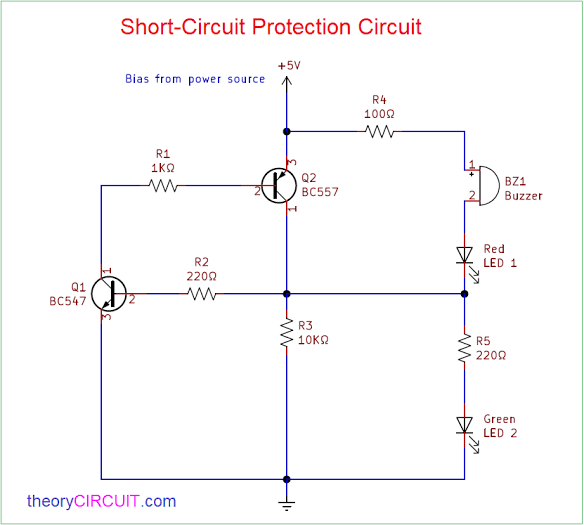
\includegraphics[scale=1.1]{jamal.png}
  \caption{Schematic diagram}
  \label{fig:image1}
 \vspace{3cm}
   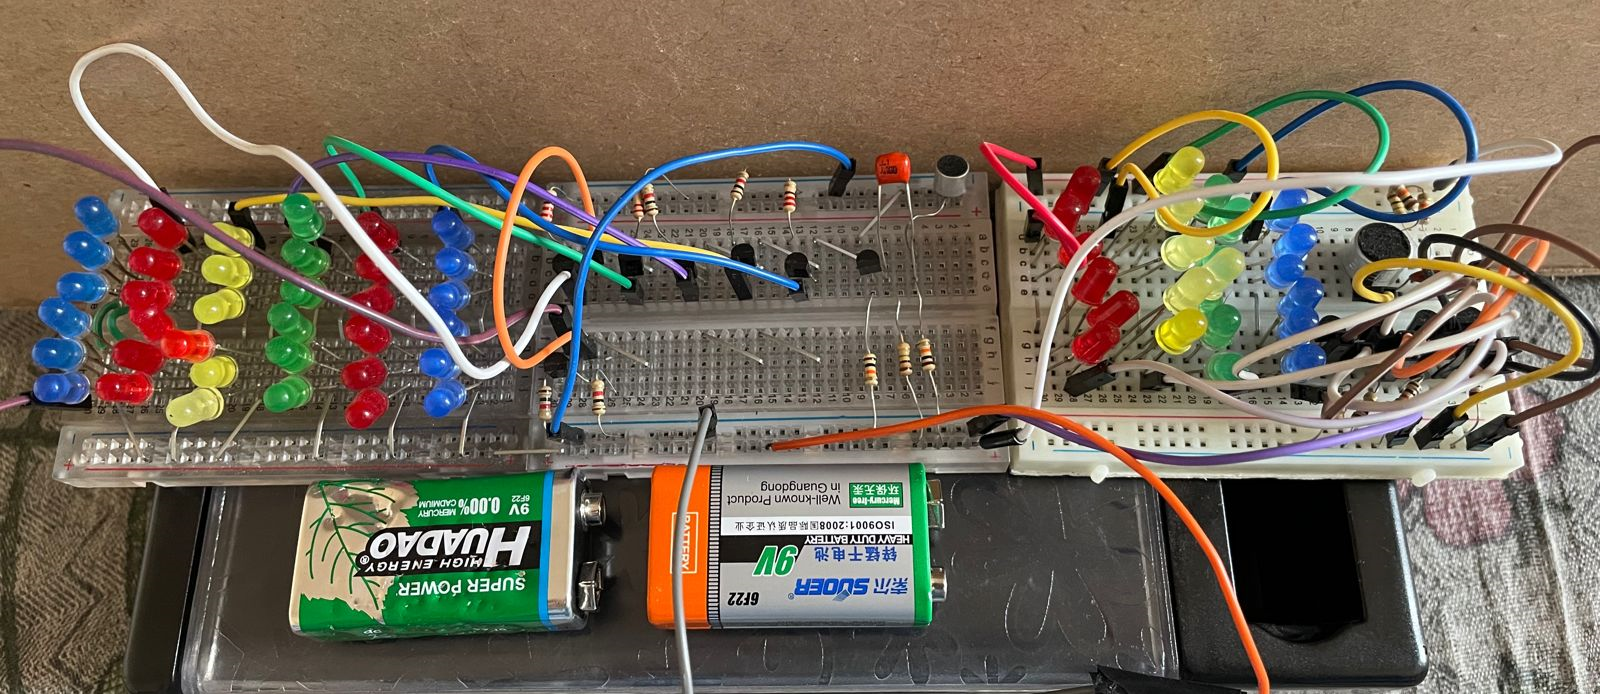
\includegraphics[scale=1.1]{PIC1.png}
  \caption{Schematic diagram}
  \label{fig:image1}
\end{figure}
\end{block}
\end{column}

% Now is the last column
\begin{column}{\sepwid}\end{column} % empty spacer column
\begin{column}{\onecolwid}
\begin{block}{\textcolor{blue}{Operating Procedure}}
\textbf  {\large operate in four steps:}

\begin{itemize}
\item \textbf{ Step 1: Monitoring}
\begin{itemize}
  \item The circuit continuously checks the electrical current flowing through it.
\end{itemize}



\item \textbf{Step 2:Threshold Detection:}
\begin{itemize}
  \item  If the current exceeds a specific limit, indicating a potential short circuit, the circuit proceeds to the next step.

\end{itemize}
\item \textbf{Step 3:Fault Identification:}
\begin{itemize}
  \item  The circuit quickly finds the faulty section or component causing the excess current, using methods like differential current analysis or impedance measurements
\end{itemize}
\item \textbf{Step 4: Current Interruption:}
\begin{itemize}
  \item  Once the fault is identified, the circuit immediately cuts off the current flow by triggering a protective device (like a fuse or circuit breaker), preventing further damage and allowing for repair.
\end{itemize}
\end{itemize}

\end{block}

\end{column} % empty spacer column

\end{columns}
\end{frame}
\end{document}

